%%【PostScript, JPEG, PNG等の画像の貼り込み】
%% 利用するパッケージを選んでコメントアウトしてください.
\usepackage{graphicx} % for 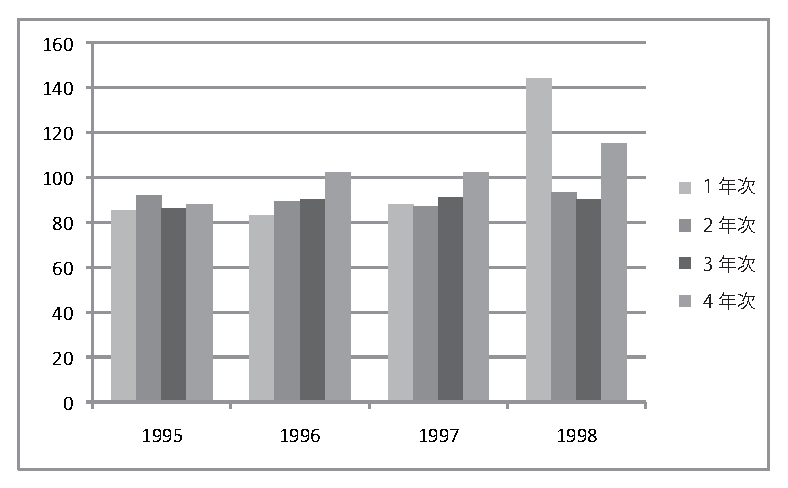
\includegraphics[width=3cm]{sample.eps}
\usepackage{epsfig} % for 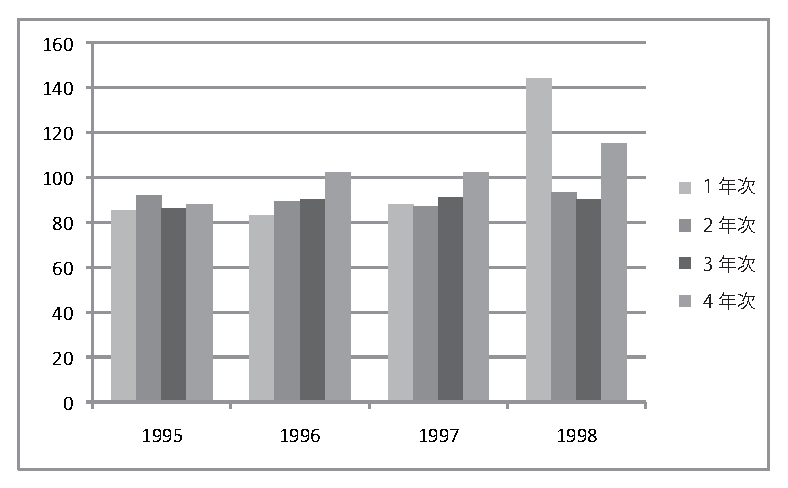
\psfig{file=sample.eps,width=3cm}
%\usepackage{epsf} % for \epsfile{file=sample.eps,scale=0.6}
%\usepackage{epsbox} % for \epsfile{file=sample.eps,scale=0.6}
\usepackage{/Users/takagihayata/workspace/materialize-mongodb/paper/mast/class/mediabb} % for pdf

\usepackage{times} % use Times Font instead of Computer Modern
% \usepackage{listings} % for soursecode
% \usepackage{plistings} % for soursecode
\usepackage{/Users/takagihayata/workspace/materialize-mongodb/paper/mast/class/docmute} % texファイル分割用

\setcounter{tocdepth}{3}
\setcounter{page}{-1}

\setlength{\oddsidemargin}{0.1in}
\setlength{\evensidemargin}{0.1in}
\setlength{\topmargin}{0in}
\setlength{\textwidth}{6in}
%\setlength{\textheight}{10.1in}
\setlength{\parskip}{0em}
\setlength{\topsep}{0em}

%\newcommand{\zu}[1]{{\gt \bf 図\ref{#1}}}

%% タイトル生成用パッケージ(重要)
\usepackage{/Users/takagihayata/workspace/materialize-mongodb/paper/mast/class/mast-jp-sjis}

%% タイトル
%% 【注意】タイトルの最後に\\ を入れるとエラーになります
\title{NoSQL型データベースシステムでの実体化ビュー選択に関する研究}
%% 著者
\author{髙木 颯汰}
%% 指導教員
\advisor{古瀬 一隆 陳 漢雄}

%% 年月 (提出年月)
%% 年月は必要に応じて書き替えてください.
\majorfield{ } \yearandmonth{2019年 1月}
